\documentclass[12pt]{article}
\usepackage[letterpaper, margin=1in]{geometry}
\usepackage{graphicx}
\usepackage{amssymb}
\usepackage{helvet}
\renewcommand{\familydefault}{\sfdefault}
\usepackage{setspace}
\usepackage{wrapfig}
\usepackage{listings}

\begin{document}
    \singlespacing
    \section*{Tache Only Data}
    \subsection*{Method}
    \indent
    \indent
    The model is tasked to check whether or not the nasal vowel was normal or clear
    speech. The architecture used was a Random Forest classifier from sklearn. The
    model has 1200 estimaters each with a depth of 10. The labels used in training
    are freq f1,amp f1,width f1, freq f2, amp f2, width f2, freq f3, amp f3, width
    f3, amp p0, freq p0, p0prominence,a1p0,a3p0,vwl amp rms,vwl duration,appendix
    dur. The timepoint, clarity, and label were dropped for the training set and the
    only column used to check the prediction was the label column. There is a
    $70\%$ $30\%$ split on the data for the training and test sets. To check how the
    model is doing, clacultions of accuract, hamming loss, F1, precision, recall,
    macro and weighted average, and classification report.
    \subsection*{Rseults}
    \begin{table}[ht!]
        \centering
        \caption{Classification Report}
        \label{table:report}
        \begin{tabular}{|l|c|c|c|c|}
            \hline
            \textbf{type} & \textbf{precision} & \textbf{recall} & \textbf{f1-score} & \textbf{support} \\
            \hline
            \hline
            $0$ (clear)   & $66\%$             & $76\%$          & $71\%$            & $140$            \\
            \hline
            $1$ (normal)  & $76\%$             & $67\%$          & $71\%$            & $162$            \\
            \hline
            accuracy      &                    &                 & $71\%$            & $302$            \\
            \hline
            macro avg     & $71\%$             & $71\%$          & $71\%$            & $302$            \\
            \hline
            weighted avg  & $71\%$             & $71\%$          & $71\%$            & $302$            \\
            \hline
        \end{tabular}
    \end{table}

    \begin{wrapfigure}
        {r}{0.5\textwidth}
        \centering
        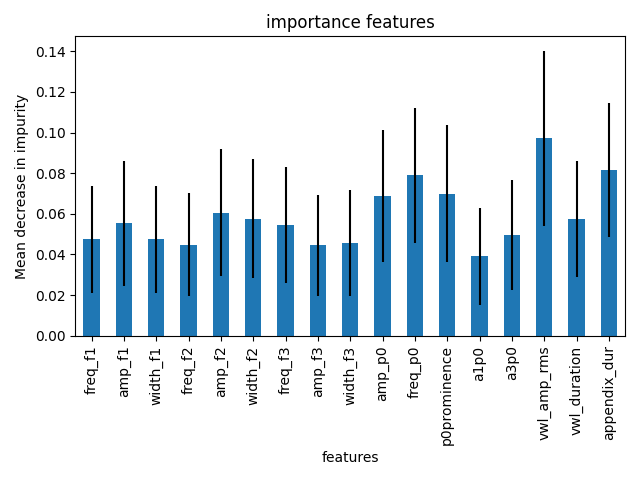
\includegraphics[width=\linewidth]{
            ../py_files/decision_tree/importance.png
        }
        \caption{Feature importances using MDI}
        \label{fig:importance}
    \end{wrapfigure}

    \indent
    \indent
    When we look at Table~\ref{table:report}, we see that the model levels off
    at around $71\%$. It is interesting to see that for the classification of normal
    speech, the precision of the model is $76\%$. It is hard to find why the model
    stabalizes at $71\%$ but this is something to look further. I also
    calculated the hamming loss and accuracy. The accuracy came out to $70.86\%$.
    The hamming loss is a metric specifically for multi-class models, like this random
    forest. According to Scikit learn, "The Hamming loss is the fraction of
    labels that are incorrectly predicted." Given that, the model had a hamming loss
    of around $0.29$ which is not desirable since we would want the loss to be as
    near $0$

    \indent
    When we look at Figure~\ref{fig:importance}, we see that all of the features play
    a role but out of the columns in the csv file, the vowel amplitude rms
    feature played the most into the decision tree prediction. The MDI stands for
    "Mean Decreased in Impurity" which, according to skilearn themselves, is computed
    by the mean and standard deviation of accumulation of the impurity decrease within
    each tree. MDI calculates the total reduction of node impurity across all of
    the trees.

    \begin{wrapfigure}
        {r}{0.5\textwidth}
        \centering
        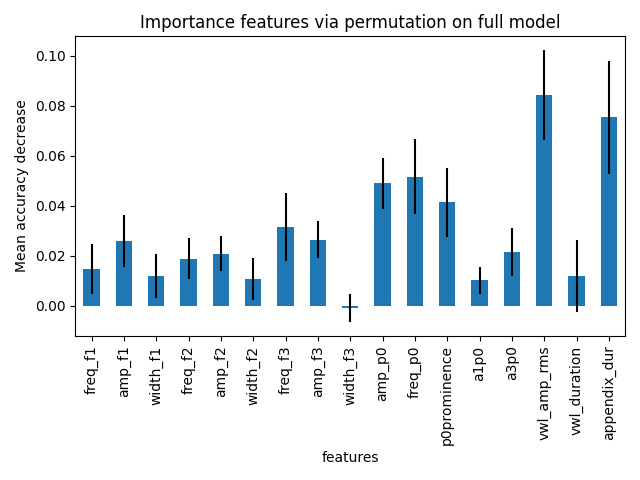
\includegraphics[width=\linewidth]{
            ../py_files/decision_tree/permutation.png
        }
        \caption{Feature importances using permutation}
        \label{fig:permunation}
    \end{wrapfigure}
    There were no one feature that solely decides the random forest that does
    the prediction. Using the MDI, shows how each feature contributes in the
    decision of the prediction. The drawback with using MDI is that it can biased
    towards numerical features or columns with many unique values.

    \indent
    Figure~\ref{fig:permunation} shows the importance of the features using permutations
    on the full model. In this case, the features are shuffled $n$ times, twice
    in Figure~\ref{fig:permunation} and the model then predicts on the shuffled
    data. This approached on contrast to the MDI importance, does not take into
    account of biases and check each feature and their contribution. We can see the
    two features that are helping the model make the predictions, being the
    vowel amplitude rms and the appendix duration.

    \section*{Tache and Lecture Data}
    \subsection*{Method}
    \indent
    \indent
    The model is tasked to check whether or not the nasal vowel was normal or
    clear speech. The architecture used was a Random Forest classifier from sklearn.
    The model has 1000 estimaters each with a depth of 30. The labels used in
    training are freq f1,amp f1,width f1, freq f2, amp f2, width f2, freq f3, amp
    f3, width f3, amp p0, freq p0, p0prominence,a1p0,a3p0,vwl amp rms,vwl duration,appendix
    dur. The search query, speaker, task, clarity, ND, timepoint, word, vowel,
    and target columns were dropped for the training set and the only column
    used to check the prediction was the label column. There is a $80\%$ $20\%$ split
    on the data for the training and test sets. To check how the model is doing, clacultions
    of accuracy on the validation set, precision, recall, F1-score, macro average,
    weighted average, and out of the box (OOB) score.

    \subsection*{Results}
    \begin{table}[ht!]
        \centering
        \caption{Classification Report}
        \label{table:tache_lecture_report}
        \begin{tabular}{|l|c|c|c|c|}
            \hline
            \textbf{type} & \textbf{precision} & \textbf{recall} & \textbf{f1-score} & \textbf{support} \\
            \hline
            \hline
            $0$ (clear)   & $80\%$             & $82\%$          & $81\%$            & $394$            \\
            \hline
            $1$ (normal)  & $82\%$             & $81\%$          & $81\%$            & $411$            \\
            \hline
            accuracy      &                    &                 & $81\%$            & $805$            \\
            \hline
            macro avg     & $81\%$             & $81\%$          & $81\%$            & $805$            \\
            \hline
            weighted avg  & $81\%$             & $81\%$          & $81\%$            & $805$            \\
            \hline
        \end{tabular}
    \end{table}

    The full report is shown in table~\ref{table:tache_lecture_report}. We can see
    the increase in all values with across the board wavering at least around $80
    \%$. This is a big gain in the classification regards compared to just the
    lecture data due to the increase of data, as we can see that for the normal has
    increased to $411$ entries to support and in the clear has increased to $394$
    entries.

    Table~\ref{table:other_results} provides the val accuracy and the OOB score.
    According to the Scikit-learn official website, the OOB score (or error from
    their website) is as follows:
    \begin{quotation}
        \noindent
        the average error for each $z_{i}= (x_{i}y_{i})$ calculated using predictions
        from the trees that do not contain $z_{i}$ in their respective bootstrap sample.
    \end{quotation}

    \begin{table}[ht!]
        \centering
        \caption{Other Report}
        \label{table:other_results}
        \begin{tabular}{|l|c|c|c|c|}
            \hline
            \textbf{type}       & \textbf{result} \\
            \hline
            \hline
            Validation accuracy & $81.12\%$       \\
            \hline
            OOB score           & $80.37\%$       \\
            \hline
        \end{tabular}
    \end{table}
    \begin{wrapfigure}
        {r}{0.5\textwidth}
        \centering
        
\includegraphics[width=\linewidth]{
            ../py_files/decision_tree/importance_with_tache.png
        }
        \caption{Feature importances using MDI}
        \label{fig:combined_importance}
    \end{wrapfigure}

    The validation accuracy is just how well the model did on the set that was
    not seen in the training set. Figure~\ref{fig:combined_importance} shows what
    feature plays a factor in the random forest.

    In this case, it is the vowel amplitude rms. We can see that the appendix duration
    is up next with the second feature that the random forest model will look at.
    Interestingly, the features of nasality does not play a role in the decision.

    \begin{wrapfigure}
        {r}{0.5\textwidth}
        \centering
        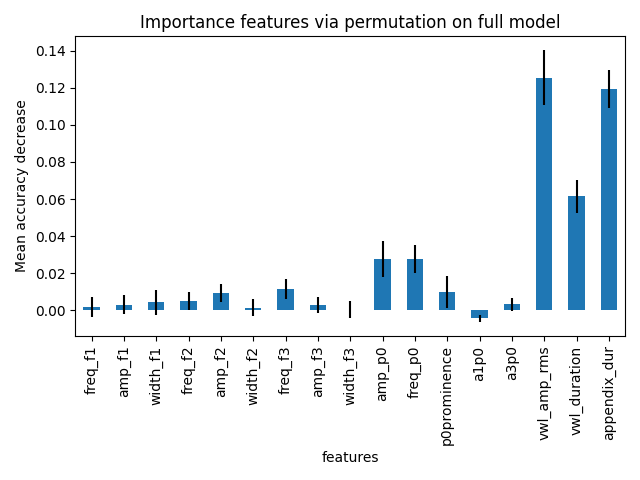
\includegraphics[width=\linewidth]{
            ../py_files/decision_tree/permutation_with_tache.png
        }
        \caption{Feature importances using permutation}
        \label{fig:combined_permunation}
    \end{wrapfigure}

    In Figure~\ref{fig:combined_permunation}, we can see how much the model relies
    on the vowel amplitude ams and the appendix duration where they are almost the
    same at $0.14$. In both figures, we can see a sharp drop in the third feature
    of the actual vowel duration, at around $0.08$. We can see in figure~\ref{fig:combined_permunation}
    that the features of nasality other than P0 are low, not reaching $0.02$. The
    amplitude and frequency of P0 is far lower in the chain of features but it is
    interesting that it comes before the formants of the vowel and a1-p0
\end{document}